\documentclass[11pt,a4paper]{article}
\usepackage[margin=2cm]{geometry}
\usepackage[T1]{fontenc}
\usepackage[utf8]{inputenc}
\usepackage{lmodern,microtype}
\usepackage{amsmath,amssymb,mathtools,bm}
\usepackage{booktabs,tabularx,longtable,array,multirow}
\usepackage{graphicx,caption,subcaption,float}
\usepackage{enumitem,xcolor,hyperref,cleveref}
\usepackage{fancyhdr,titlesec,siunitx,url}
\usepackage[most]{tcolorbox}
\usepackage{tikz}
\usetikzlibrary{arrows.meta,positioning,fit,calc,shapes.geometric,backgrounds}

\definecolor{deepblue}{RGB}{28,63,105}
\definecolor{deepgreen}{RGB}{38,105,79}
\definecolor{deeporange}{RGB}{170,92,20}
\definecolor{deepred}{RGB}{145,52,52}
\definecolor{softblue}{RGB}{232,241,250}
\definecolor{softgreen}{RGB}{235,247,240}
\definecolor{softorange}{RGB}{253,243,226}
\definecolor{softred}{RGB}{252,235,235}
\definecolor{softgray}{RGB}{245,246,248}
\hypersetup{
 colorlinks=true,
 linkcolor=deepblue,
 citecolor=deepgreen,
 urlcolor=deeporange,
 pdftitle={Geometry-MMALS G1 v1.1.2: Smooth Residual and SPD Results},
 pdfauthor={Guillaume Harbonnier}
}
\pagestyle{fancy}\fancyhf{}
\lhead{Geometry-MMALS G1}
\rhead{v1.1.2 five-seed results}
\cfoot{\thepage}
\setlength{\headheight}{14pt}
\titleformat{\section}{\Large\bfseries\color{deepblue}}{\thesection}{0.8em}{}
\titleformat{\subsection}{\large\bfseries\color{deepgreen}}{\thesubsection}{0.8em}{}
\titleformat{\subsubsection}{\normalsize\bfseries\color{deeporange}}{\thesubsubsection}{0.8em}{}
\setlist[itemize]{leftmargin=1.5em,itemsep=2pt,topsep=3pt}
\setlist[enumerate]{leftmargin=1.7em,itemsep=3pt,topsep=3pt}
\renewcommand{\arraystretch}{1.14}
\newcolumntype{Y}{>{\raggedright\arraybackslash}X}
\newcolumntype{C}{>{\centering\arraybackslash}X}
\newcommand{\MMALS}{\textsc{MMALS}}
\newcommand{\R}{\mathbb{R}}
\newcommand{\E}{\mathbb{E}}
\newcommand{\loss}{\mathcal{L}}
\newcommand{\norm}[1]{\left\lVert #1 \right\rVert}
\newcommand{\softmax}{\operatorname{softmax}}
\newcommand{\OT}{\operatorname{OT}}
\newtcolorbox{plainbox}[1][]{title={#1},colback=softblue,colframe=deepblue!45,boxrule=.6pt,arc=2pt,left=8pt,right=8pt,top=7pt,bottom=7pt}
\newtcolorbox{positivebox}[1][]{title={#1},colback=softgreen,colframe=deepgreen!45,boxrule=.6pt,arc=2pt,left=8pt,right=8pt,top=7pt,bottom=7pt}
\newtcolorbox{warningbox}[1][]{title={#1},colback=softorange,colframe=deeporange!50,boxrule=.6pt,arc=2pt,left=8pt,right=8pt,top=7pt,bottom=7pt}
\newtcolorbox{criticalbox}[1][]{title={#1},colback=softred,colframe=deepred!50,boxrule=.6pt,arc=2pt,left=8pt,right=8pt,top=7pt,bottom=7pt}
\newtcolorbox{mathbox}[1][]{title={#1},colback=softgray,colframe=black!30,boxrule=.5pt,arc=1pt,left=8pt,right=8pt,top=7pt,bottom=7pt}

\begin{document}
\begin{titlepage}
\centering
\vspace*{0.4cm}
{\Huge\bfseries\color{deepblue} Geometry-MMALS G1 v1.1.2\par}
\vspace{0.25cm}
{\LARGE Smooth Simplex-Residual Routing\par}
\vspace{0.08cm}
{\LARGE and Covariance-Aware Context Diagnostics\par}
\vspace{0.45cm}
{\Large Five-seed results, corrected manifests, falsification outcome, and reviewer-facing interpretation\par}
\vspace{0.7cm}
{\Large Guillaume Harbonnier\par}
\vspace{0.15cm}
{\normalsize Independent MMALS research program\par}
\vspace{0.15cm}
{\normalsize \href{https://github.com/gharbonnier78/geometry-mmalls-g1}{github.com/gharbonnier78/geometry-mmalls-g1}\par}
\vspace{0.55cm}
{\normalsize RotatedMNIST pilot, five matched-compute seeds, June 2026\par}
\vfill
\begin{minipage}{0.94\textwidth}\small
\textbf{Epistemic status.} The five-seed pilot completed for seeds 0--4 under the frozen bridge-isolation protocol. The primary R5 smooth-residual router did not qualify against the preregistered R1 linear structural reference: held-out functional order, held-out functional stress, continuity non-degradation, causal specificity, and operational non-degradation did not all pass. However, R5 is consistently more ordered and lower-stress than the flexible R0 MLP router, route-swap ordering passes, and the sharp local tails of R3 are removed. The covariance-aware SPD diagnostic also passes: the combined centroid-plus-Log-Euclidean context metric reduces stress relative to centroid-only geometry in all five seeds. This SPD result is diagnostic and does not establish a learned Riemannian manifold.
\end{minipage}
\vfill
\end{titlepage}

\begin{abstract}
Geometry-MMALS asks whether an inferred context geometry can organize routing through a modular host ecosystem in a functionally meaningful and auditable way. Version 1.1.2 preserves the strict bridge-isolation controls of v1.1.1: within each seed, the sensory encoder, four-dimensional context encoder, host bank, synthesis normalization, classifier, and common host-functional cost matrix are frozen and shared across all router treatments. We compare six matched-compute routers: a flexible MLP (R0), a linear router (R1), prototype energy (R2), directional-prototype hybrid energy (R3), a bounded smooth residual router (R4), and the same router with a context-only simplex-continuity hinge (R5).

The primary R5-versus-R1 held-out functional effects are small and non-qualifying. Functional distance-order correlation changes by $+0.0109$ with 95\% seed interval $[-0.0487,0.0705]$, and functional stress changes by $-0.0179$ with interval $[-0.0671,0.0314]$. Local functional continuity q95 is nearly identical on average for R5 and R1 ($0.2693$ versus $0.2713$), but the paired seed interval $[-0.1702,0.1663]$ exceeds the preregistered non-degradation tolerance. Causal specificity fails because only three of five seeds have a minimum lower bootstrap bound above one, despite mean functional CSR $1.780$. Operational non-degradation fails: R5 loses $0.964$ percentage points of held-out accuracy and $0.894$ points of final trained accuracy relative to R0, although forgetting improves by $0.169$ points.

Two narrower results survive. First, R5 significantly improves over R0 on held-out common-cost functional geometry: $\Delta\rho=+0.0496$ with interval $[0.0243,0.0748]$ and $\Delta$stress $=-0.0394$ with interval $[-0.0592,-0.0196]$. Second, R5 reduces the severe R3 continuity q95 by $1.676$ on average without losing held-out functional geometry. The smooth repair therefore removes prototype sharpness but adds no robust value beyond the linear router. Separately, covariance-aware context diagnostics pass: centroid-plus-Log-Euclidean stress improves by $-0.0442$ with interval $[-0.0638,-0.0246]$ and a favorable fraction of $5/5$ seeds. The result redirects the program away from additional router complexity and toward route-function memory transport and causal host-bank alignment.
\end{abstract}

\tableofcontents
\clearpage

\section{Reviewer decision summary}
\begin{criticalbox}[Primary decision]
\textbf{The R5 smooth-residual router does not qualify.} The failure is scientific rather than procedural: the common components are exactly frozen, compute is matched, and all five seeds completed. The primary R5-versus-R1 structural comparison does not establish a robust gain in held-out functional order, functional stress, or local continuity, and the operational equivalence gate fails against R0.
\end{criticalbox}

\begin{positivebox}[What survives]
Three narrower findings are supported. R5 outperforms R0 on held-out route geometry; R5 removes the severe local sensitivity of R3; and covariance-aware context geometry adds stable factor information beyond centroid-only geometry. These findings constrain the next experiment even though they do not qualify R5 as the preferred router.
\end{positivebox}

\begin{table}[H]
\centering
\caption{Reviewer-facing gate outcome. A failed gate means the preregistered threshold was not met, not that the software or execution failed.}
\label{tab:gates}
\small
\begin{tabularx}{\textwidth}{@{}Y c Y@{}}
\toprule
Gate & Outcome & Interpretation \\
\midrule
Context and common host bank frozen & Pass & Exact zero context and host-output deltas across treatments. \\
Equal router compute & Pass & 15,360 forward images and 80 optimizer steps per method and seed. \\
Held-out functional stress reduction vs R1 & Fail & Mean favorable, but seed interval crosses zero. \\
Held-out functional order vs R1 & Fail & Mean favorable, but seed interval crosses zero. \\
Local continuity non-degradation vs R1 & Fail & Mean nearly equal, but the paired upper interval exceeds tolerance. \\
Route-swap order & Pass & Far swaps exceed near swaps for every R5 seed. \\
Functional causal specificity & Fail & Only three of five seeds have lower CSR bound above one. \\
Prediction identity preservation & Pass & Minimum per-seed preservation is 0.981. \\
Operational non-degradation vs R0 & Fail & Too few seeds remain within the one-point held-out margin. \\
SPD covariance adds value & Pass, diagnostic & Combined covariance-aware stress improves in all five seeds. \\
Mature host specialization & Not tested & Hosts are frozen; only allocation is observed. \\
Memory transport & Not implemented & Deferred to v1.1.3. \\
Operational superiority & Not claimed & Not preregistered as a primary claim. \\
\bottomrule
\end{tabularx}
\end{table}

\subsection{Manifest correction}
The numerical run completed, but the original \texttt{claim\_manifest.json} retained the pre-execution string \texttt{pilot\_pending}. The release corrects this to \texttt{five\_seed\_pilot\_completed}, records \texttt{r5\_smooth\_residual\_router\_not\_qualified}, and records \texttt{spd\_covariance\_adds\_value\_candidate\_supported}. This is a metadata-only correction. No CSV value, checkpoint hash, cost matrix, gate, or source split changed.

\section{Scientific question and controlled design}
\subsection{Why v1.1.2 exists}
Version 1.1.1 established a clean bridge-isolation protocol but rejected the prototype-dominated R3 router. The main failure mode was not an absence of route structure. R3 and R2 reduced functional stress and produced ordered far-versus-near route swaps. The dominant problem was excessive local sensitivity: small context movements produced large route changes. Version 1.1.2 therefore tests whether a bounded residual and a context-only continuity hinge can preserve route structure without recreating the sharp local tails.

The central question is deliberately narrow:
\begin{quote}
Given the same frozen context, the same fixed host functions, and the same common functional cost, does a linear-first bounded residual router improve held-out functional route geometry while remaining as smooth as the linear router and as operationally safe as the MLP router?
\end{quote}

\subsection{Frozen causal chain}
\begin{figure}[H]
\centering
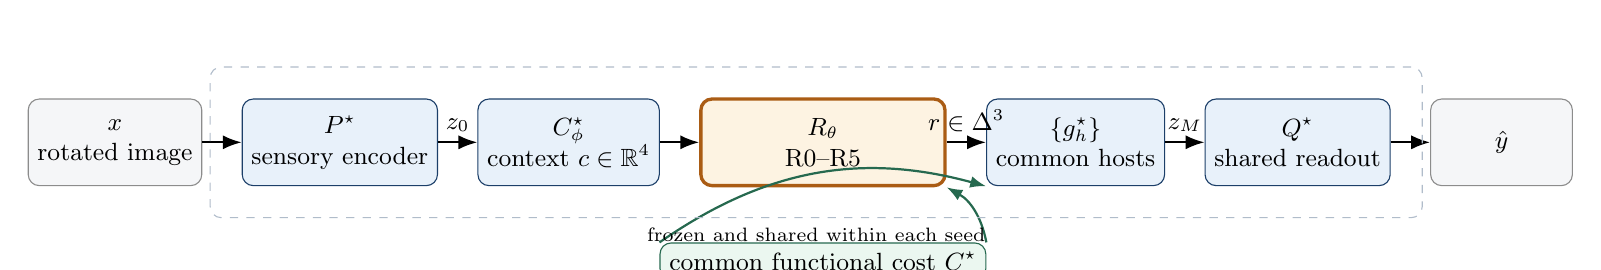
\begin{tikzpicture}[
 node distance=5mm and 5mm,
 every node/.style={font=\small,align=center},
 frozen/.style={draw=deepblue,fill=softblue,rounded corners,minimum height=11mm,minimum width=22mm},
 trainable/.style={draw=deeporange,fill=softorange,rounded corners,minimum height=11mm,minimum width=31mm,very thick},
 data/.style={draw=black!45,fill=softgray,rounded corners,minimum height=11mm,minimum width=18mm},
 arrow/.style={-{Latex[length=2.4mm]},thick}
]
\node[data] (x) {$x$\\rotated image};
\node[frozen,right=of x] (p) {$P^\star$\\sensory encoder};
\node[frozen,right=of p] (c) {$C_\phi^\star$\\context $c\in\R^4$};
\node[trainable,right=of c] (r) {$R_\theta$\\R0--R5};
\node[frozen,right=of r] (h) {$\{g_h^\star\}$\\common hosts};
\node[frozen,right=of h] (q) {$Q^\star$\\shared readout};
\node[data,right=of q] (y) {$\hat y$};
\draw[arrow] (x)--(p);
\draw[arrow] (p)--node[above]{$z_0$}(c);
\draw[arrow] (c)--(r);
\draw[arrow] (r)--node[above]{$r\in\Delta^3$}(h);
\draw[arrow] (h)--node[above]{$z_M$}(q);
\draw[arrow] (q)--(y);
\node[below=7mm of r,draw=deepgreen,fill=softgreen,rounded corners,minimum width=40mm] (cost) {common functional cost $C^\star$};
\draw[-{Latex[length=2mm]},deepgreen,thick] (cost.north west) to[bend left=25] (h.south west);
\draw[-{Latex[length=2mm]},deepgreen,thick] (cost.north east) to[bend right=25] (r.south east);
\node[fit=(p)(c)(h)(q),draw=deepblue!35,dashed,rounded corners,inner sep=4mm,label=below:{\scriptsize frozen and shared within each seed}] {};
\end{tikzpicture}
\caption{v1.1.2 bridge isolation. Only router parameters differ during the treatment comparison.}
\label{fig:architecture}
\end{figure}

\subsection{Six router treatments}
\begin{table}[H]
\centering
\caption{Router treatments and trainable parameter counts.}
\small
\begin{tabularx}{\textwidth}{@{}l r Y@{}}
\toprule
Router & Parameters & Role \\
\midrule
R0 MLP & 4,740 & Flexible operational reference. \\
R1 linear & 20 & Low-capacity smooth structural reference. \\
R2 prototype energy & 24 & Local prototype territories. \\
R3 hybrid energy & 42 & Directional plus prototype control from v1.1.1. \\
R4 smooth residual & 141 & Linear base plus bounded prototype residual. \\
R5 smooth residual + continuity & 141 & R4 with context-only simplex-continuity hinge. \\
\bottomrule
\end{tabularx}
\end{table}

\section{Mathematical objects}
\subsection{Route simplex}
For four hosts, the route satisfies
\begin{equation}
 r=(r_1,r_2,r_3,r_4)\in\Delta^3,
 \qquad r_h\ge 0,
 \qquad \sum_{h=1}^{4}r_h=1.
\end{equation}
The nominal distance uses the square-root simplex embedding:
\begin{equation}
 d_R(r_a,r_b)=\frac{\norm{\sqrt{r_a}-\sqrt{r_b}}_2}{\sqrt{2}}.
\end{equation}
This is a Hellinger-type distance rather than a Euclidean distance between unconstrained logits.

\subsection{Common functional route distance}
A route is interpreted through the frozen host ecosystem. Let $C^\star_{hk}$ denote the normalized output distance between hosts $h$ and $k$. The functional route distance is an entropically regularized optimal-transport cost
\begin{equation}
 d_F(r_a,r_b)=\OT_{C^\star,\varepsilon}(r_a,r_b).
\end{equation}
Every treatment is evaluated with the same $C^\star$ within a seed. This is essential: otherwise a router could appear geometrically different simply because it trained a different host bank.

\subsection{Smooth residual router}
R4 and R5 start from a linear base
\begin{equation}
 \ell^{\mathrm{base}}(c)=Wc+b.
\end{equation}
Prototype evidence is centered, normalized, and bounded:
\begin{equation}
 \delta_h(c)=\tanh\!\left(
 \frac{s_h(c)-\overline{s}(c)}{\operatorname{Std}_k s_k(c)+\epsilon}
 \right),
 \qquad |\delta_h(c)|\le 1.
\end{equation}
A gate $g(c)\in[0,1]$ controls when the residual is active, and the residual amplitude is capped by $s_{\max}$:
\begin{equation}
 r(c)=\softmax\!\left(Wc+b+s_{\max}g(c)\delta(c)\right).
\end{equation}
R5 adds a factor-label-free continuity hinge
\begin{equation}
 \loss_{\mathrm{cont}}=
 \E\left[
 \max\left(
 0,
 d_R(r_a,r_b)-\kappa d_C(c_a,c_b)-m
 \right)^2
 \right].
\end{equation}
The hinge uses only inferred contexts and routes; it does not use the ground-truth rotation angle.

\subsection{Covariance-aware context geometry}
For each angle $u$, context vectors across source identities define a regularized covariance
\begin{equation}
 \Sigma_u=(1-\lambda)\widehat{\operatorname{Cov}}(c\mid u)
 +\lambda\frac{\operatorname{tr}(\widehat\Sigma_u)}{d}I+\epsilon I.
\end{equation}
The diagnostic compares centroid distance with three SPD distances:
\begin{align}
 d_{\mathrm{LE}}(\Sigma_u,\Sigma_v)
 &=\norm{\log\Sigma_u-\log\Sigma_v}_F,\\
 d_{\mathrm{AIRM}}(\Sigma_u,\Sigma_v)
 &=\norm{\log(\Sigma_u^{-1/2}\Sigma_v\Sigma_u^{-1/2})}_F,\\
 d_{\mathrm{BW}}^2(\Sigma_u,\Sigma_v)
 &=\operatorname{tr}\!\left(\Sigma_u+\Sigma_v
 -2(\Sigma_u^{1/2}\Sigma_v\Sigma_u^{1/2})^{1/2}\right).
\end{align}
The preregistered SPD candidate combines normalized centroid and Log-Euclidean distances. This axis is diagnostic; it does not claim that the network learned a global Riemannian manifold.

\section{Protocol and statistics}
The pilot uses model seeds 0--4. Every router receives 15,360 forward images and 80 optimizer steps. Source identities are split into disjoint partitions for common-cost construction, probe fitting, probe evaluation, tangent fitting, causal evaluation, and route-swap evaluation. Per-source geometry effects are bootstrapped within seed. Across seeds, mean effects use a Student-$t$ interval with $n=5$.

The primary structural contrast is R5 versus R1. R5 versus R0 is an operational and secondary geometric comparison. R5 versus R3 tests whether the repair removes sharpness without destroying the geometry that motivated the prototype family.

\section{Primary router result}
\subsection{R5 does not robustly improve on R1}
The primary held-out functional effects are
\begin{align}
 \Delta\rho_{R5-R1}&=+0.010886,
 &95\%\ \mathrm{CI}&=[-0.048685,0.070456],\\
 \Delta\mathrm{stress}_{R5-R1}&=-0.017859,
 &95\%\ \mathrm{CI}&=[-0.067115,0.031396].
\end{align}
The point estimates are favorable, but both intervals cross zero. The favorable seed fraction is $3/5$ for correlation and $4/5$ for stress. Under the preregistered rule, neither effect qualifies.

R4 also fails to improve on R1: its held-out functional correlation effect is $-0.00435$ with interval $[-0.07597,0.06728]$, and stress effect is $-0.00050$ with interval $[-0.04803,0.04703]$. The bounded residual alone therefore adds no measurable structural value over the linear route.

\begin{figure}[H]
\centering
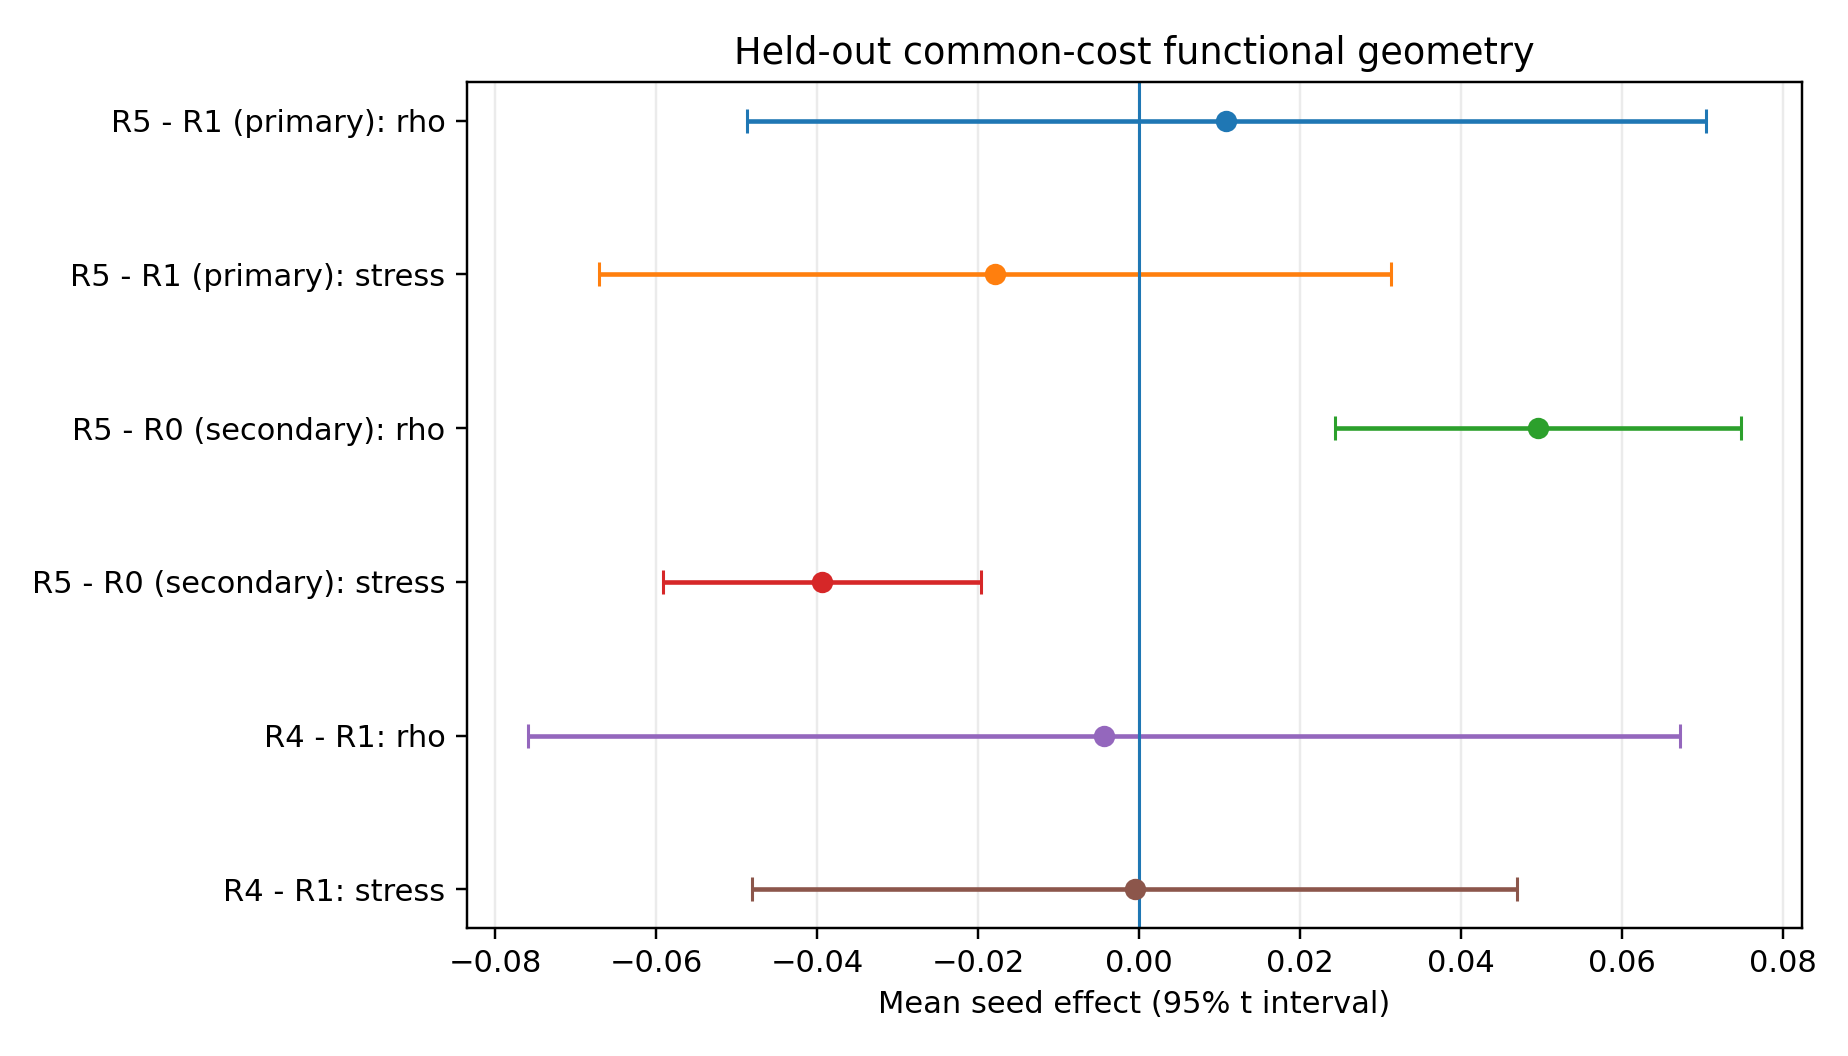
\includegraphics[width=0.93\textwidth]{figures/heldout_functional_effects.png}
\caption{Held-out common-cost functional effects. For correlation, positive is favorable; for stress, negative is favorable. The R5-versus-R1 primary intervals cross zero. R5-versus-R0 is consistently favorable.}
\label{fig:effects}
\end{figure}

\subsection{R5 significantly improves on R0}
The secondary R5-versus-R0 comparison is unambiguously favorable:
\begin{align}
 \Delta\rho_{R5-R0}&=+0.049574,
 &95\%\ \mathrm{CI}&=[0.024319,0.074828],\\
 \Delta\mathrm{stress}_{R5-R0}&=-0.039398,
 &95\%\ \mathrm{CI}&=[-0.059165,-0.019631].
\end{align}
All five seeds favor R5. This matters, but it does not rescue the primary claim. The correct interpretation is that the structured low-capacity family is more geometrically ordered than the flexible MLP, while the smooth residual does not improve robustly beyond the linear router.

\begin{plainbox}[Reviewer interpretation]
The result is not ``R5 does nothing.'' It is ``R5 does not beat the simplest structured router.'' The linear bridge already captures most of the measurable context-to-route order. The residual and continuity machinery reduce sharpness but do not add robust held-out order beyond that baseline.
\end{plainbox}

\section{Continuity repair}
The sharpness repair succeeds relative to R3. Mean held-out functional continuity q95 values are
\begin{center}
\begin{tabular}{lr}
\toprule
Router & Mean q95 \\
\midrule
R5 residual + continuity & 0.2693 \\
R1 linear & 0.2713 \\
R4 residual & 0.3108 \\
R0 MLP & 0.3436 \\
R2 prototype & 1.7180 \\
R3 hybrid & 1.9449 \\
\bottomrule
\end{tabular}
\end{center}
R5 reduces R3 q95 by $1.6755$ on average with paired interval $[-1.7964,-1.5547]$. This is a clear mechanistic repair. Against R4, R5 reduces q95 by $0.0414$ on average, but the interval $[-0.0903,0.0074]$ still crosses zero.

Against the primary R1 reference, the mean difference is almost zero:
\begin{equation}
 \Delta q95_{R5-R1}=-0.001924,
 \qquad 95\%\ \mathrm{CI}=[-0.170151,0.166303].
\end{equation}
The upper interval exceeds the preregistered tolerance of $0.10$, so the continuity non-degradation gate fails. Two seeds show R5 worse than R1, including one large positive deviation.

\begin{figure}[H]
\centering

\includegraphics[width=0.92\textwidth]{figures/continuity_q95.png}
\caption{Held-out functional continuity q95. Dots are individual seeds; bars are means. R5 removes the R3/R2 sharpness but is not robustly non-degrading relative to R1.}
\label{fig:continuity}
\end{figure}

\section{Route swaps and causal interventions}
\subsection{Route-swap ordering passes}
For R5, mean functional route distance is $0.05147$ for near swaps and $0.11029$ for far swaps, a ratio of $2.143$. Far exceeds near in all five seeds. This supports a narrow causal-structural statement: the learned routes are not arbitrary labels, because swapping a route across a larger factor gap creates a larger functional displacement under the common host cost.

\begin{figure}[H]
\centering

\includegraphics[width=0.92\textwidth]{figures/route_swap_order.png}
\caption{Mean functional distance for near and far route swaps. The ordering passes for R5, but swap order alone does not prove tangent-specific causal mediation.}
\label{fig:swaps}
\end{figure}

\subsection{Causal specificity fails}
The causal specificity ratio compares route change under a fitted factor tangent with matched orthogonal controls. R5 mean functional CSR values by seed are $5.165$, $0.430$, $1.676$, $1.620$, and $0.010$. The overall mean is $1.780$, but the preregistered gate requires at least four of five seeds to have a lower bootstrap bound above one. Only seeds 0, 2, and 3 satisfy that condition. Seeds 1 and 4 show near-zero or sub-control specificity.

Prediction identity preservation is stable: the minimum per-seed preservation is $0.9811$, so the identity gate passes. This combination means that interventions are usually small enough not to change the class, but their direction-specific functional effect is not stable across seeds.

\begin{figure}[H]
\centering

\includegraphics[width=0.82\textwidth]{figures/causal_csr.png}
\caption{R5 causal specificity. Bars show mean CSR; triangles show the minimum lower bootstrap bound across intervention scales.}
\label{fig:causal}
\end{figure}

\section{Operational metrics}
R5 mean held-out accuracy is $0.56130$ versus $0.57094$ for R0, a loss of $0.00964$ or $0.964$ percentage points. The mean lies just inside the one-point equivalence margin, but equivalence is evaluated per seed: only two of five seeds remain within the margin. Final trained accuracy decreases by $0.00894$ on average. Forgetting improves from $0.00200$ for R0 to $0.000313$ for R5, an improvement of $0.00169$ or $0.169$ percentage points.

The result therefore exposes a familiar tradeoff: the structured route is more stable and forgets less, but the shared frozen ecosystem loses classification accuracy. Since the preregistered operational gate requires both safety and structural evidence, the reduction in forgetting cannot compensate for the accuracy failures.

\begin{figure}[H]
\centering

\includegraphics[width=0.98\textwidth]{figures/operational_summary.png}
\caption{Five-seed operational metrics. Error bars are 95\% seed intervals. R5 has low forgetting but lower accuracy than R0.}
\label{fig:operational}
\end{figure}

\section{Covariance-aware context diagnostic}
The SPD diagnostic is the clearest positive v1.1.2 result. Across seeds, centroid-only context geometry has mean $\rho=0.5394$, stress $0.4898$, and near/far AUC $0.8568$. The combined centroid-plus-Log-Euclidean metric has mean $\rho=0.6145$, stress $0.4456$, and AUC $0.9060$.

The preregistered stress contrast is
\begin{equation}
 \Delta\mathrm{stress}_{\mathrm{combined-centroid}}
 =-0.044204,
 \qquad 95\%\ \mathrm{CI}=[-0.063801,-0.024607],
\end{equation}
with all five seeds favorable. Pure Log-Euclidean, AIRM, and Bures-Wasserstein distances have even lower mean stress, approximately $0.410$, but the combined metric was the preregistered candidate because it retains both centroid displacement and covariance change.

\begin{figure}[H]
\centering
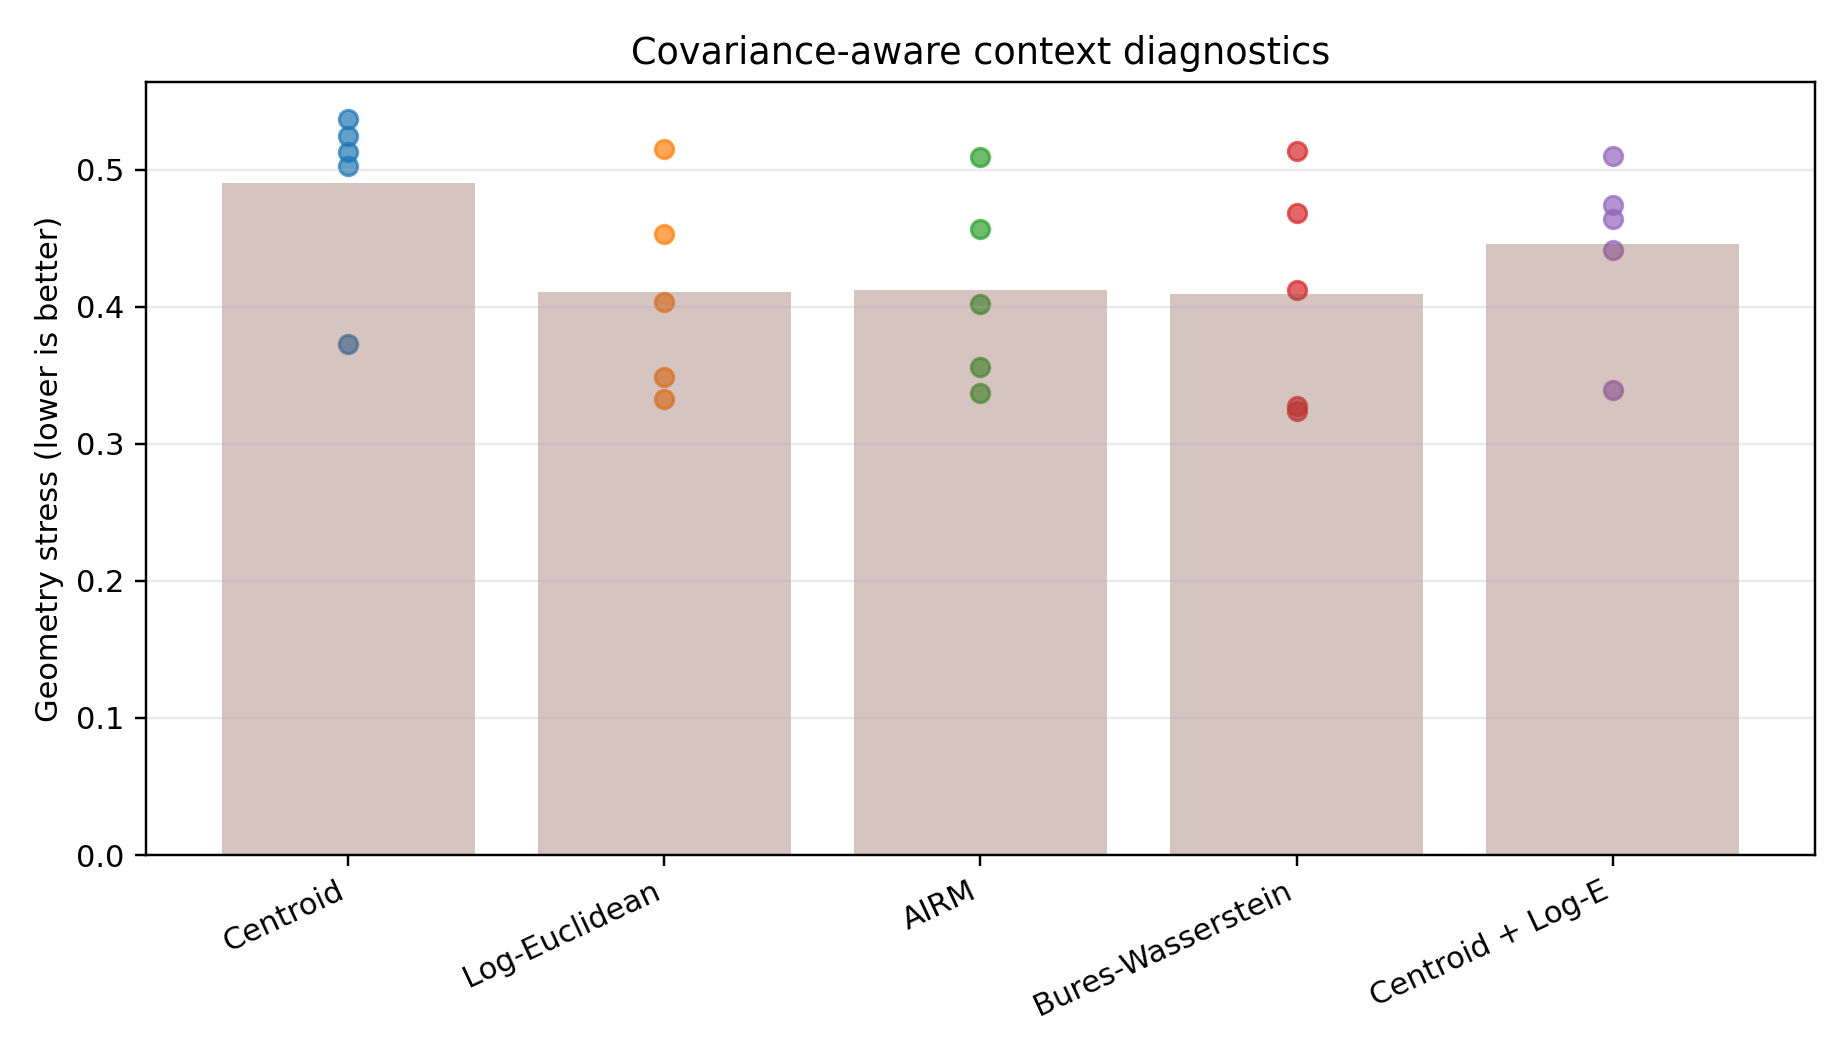
\includegraphics[width=0.92\textwidth]{figures/spd_geometry_stress.png}
\caption{Context-geometry stress by metric and seed. Covariance-aware metrics generally reduce stress. The combined candidate improves over centroid-only geometry in all five seeds.}
\label{fig:spd}
\end{figure}

\begin{warningbox}[Claim boundary]
The SPD result supports only the statement that context covariance contains stable factor information beyond the centroid. It does not show that the router uses this information, that the context space is globally Riemannian, or that an SPD-aware router would improve continual learning.
\end{warningbox}

\section{Simplex trajectories and host allocation}
The route trajectories provide a visual explanation of the quantitative results. Prototype routers produce larger territorial motions. R5 lies closer to the compact linear/MLP region than R3, while retaining a more structured progression than R0 in several seeds.

\begin{figure}[H]
\centering

\includegraphics[width=0.9\textwidth]{figures/simplex_trajectories_seed0.png}
\caption{Seed-0 mean route vectors projected to two principal components. The data remain simplex-valued in four dimensions; PCA is used only for visualization.}
\label{fig:simplex}
\end{figure}

Because hosts are frozen, these trajectories describe allocation territories, not learned host specialization. A router may consistently allocate factor regimes to different hosts even when those hosts were not causally specialized by the current stage. The report therefore keeps mature host specialization as not tested.

\section{What v1.1.2 contributes}
\subsection{Positive contributions}
\begin{enumerate}
\item It confirms that the v1.1.1 isolation protocol is reproducible with six router treatments.
\item It demonstrates that the sharp prototype continuity failure can be repaired by a bounded residual plus continuity hinge.
\item It shows that R5 and R1 are both significantly more ordered than the flexible MLP on common-cost held-out geometry.
\item It preserves route-swap ordering and prediction identity.
\item It establishes a stable covariance-aware context diagnostic across all five seeds.
\end{enumerate}

\subsection{Negative contributions}
\begin{enumerate}
\item The residual adds no robust geometry beyond the linear router.
\item The continuity hinge is seed-unstable relative to R1.
\item Tangent-specific causal mediation remains unstable.
\item The fixed ecosystem loses accuracy relative to R0.
\item Better context geometry does not automatically become better functional routing.
\end{enumerate}

\section{Implications for the MMALS architecture}
The two consecutive router studies now constrain the design space. v1.1.1 showed that strong prototypes are too sharp. v1.1.2 showed that smoothing those prototypes returns the system close to the linear baseline without producing a new robust gain. The immediate problem is therefore unlikely to be solved by adding another router term.

Three deeper hypotheses remain:
\begin{enumerate}
\item \textbf{Host-bank insufficiency.} The frozen common bank may not contain functionally distinct transformations aligned with the context factor.
\item \textbf{Readout insensitivity.} The shared classifier may not translate route differences into sufficiently useful output differences.
\item \textbf{Credit mismatch.} Classification and retention losses may not provide the router with causal allocation credit, even when context geometry is ordered.
\end{enumerate}

These hypotheses correspond directly to earlier MMALS ideas about bidirectional information flow. The next stage should not immediately unfreeze everything. It should introduce controlled diagnostics of host usefulness, route-function transport, and selective host adaptation while preserving matched-compute and source-disjoint evaluation.

\section{Recommended roadmap}
\subsection{v1.1.3: route-function memory transport}
The positive SPD diagnostic should be used to characterize memory trajectories, not to create another untested router. Let $\mu_t$ denote the distribution of route-function states after learning stage $t$. A transport diagnostic can ask how much work moves old memory into new memory:
\begin{equation}
 \mathcal{T}_{c}(\mu_t,\mu_{t+1})
 =\inf_{\gamma\in\Pi(\mu_t,\mu_{t+1})}
 \int c(u,v)\,d\gamma(u,v).
\end{equation}
The cost should separate route-only, latent-functional, behavioral, and hybrid components. This tests whether large transport predicts forgetting and whether path reconstruction is possible.

\subsection{v1.1.4: selective causal host adaptation}
The frozen-bank experiment cannot establish mature specialization. A later stage should selectively unfreeze hosts under explicit contribution and recovery controls. The core test is whether the host with the largest route allocation also has the largest causal ablation effect and whether targeted adaptation improves that alignment without destroying retention.

\subsection{G2.1 and TPUT}
Explicit host-to-router feedback and goal-conditioned control remain future layers. They should be introduced only after the program can measure host confidence, novelty, capacity, and contribution independently. Otherwise, feedback would add another controller without resolving the current functional bottleneck.

\section{Claims and non-claims}
\begin{longtable}{@{}p{0.42\textwidth}p{0.16\textwidth}p{0.34\textwidth}@{}}
\toprule
Statement & Status & Evidence boundary \\
\midrule
\endfirsthead
\toprule
Statement & Status & Evidence boundary \\
\midrule
\endhead
Common context and host bank are identical across routers & Supported & Exact preservation audit, five seeds. \\
Router compute is matched & Supported & Equal forward images and optimizer steps. \\
R5 improves held-out functional geometry over R0 & Supported, secondary & Both seed intervals exclude zero. \\
R5 improves held-out functional geometry over R1 & Not supported & Primary intervals cross zero. \\
R5 removes R3 continuity sharpness & Supported, mechanistic & Large negative paired q95 difference. \\
R5 is non-degrading in continuity relative to R1 & Not supported & Upper paired interval exceeds tolerance. \\
Far route swaps exceed near route swaps & Supported & All five R5 seeds. \\
R5 has stable tangent-specific causal mediation & Not supported & Only three of five seeds meet lower-bound criterion. \\
R5 preserves prediction identity under small interventions & Supported & Minimum preservation above 0.98. \\
R5 is operationally non-degrading relative to R0 & Not supported & Per-seed accuracy margin fails. \\
Covariance adds context-geometry information & Supported, diagnostic & Combined stress improves in all five seeds. \\
MMALS learned a Riemannian manifold & Not claimed & SPD matrices are post-hoc diagnostics. \\
Hosts are mature specialists & Not tested & Hosts are frozen. \\
Memory transport reduces forgetting & Not tested & Deferred to v1.1.3. \\
Operational superiority & Not claimed & Not preregistered. \\
Quantum advantage & Not claimed & Outside the experiment. \\
\bottomrule
\end{longtable}

\section{Limitations}
The pilot uses RotatedMNIST, five model seeds, and a four-dimensional inferred context. The host bank and classifier are deliberately frozen, which improves causal isolation but can reduce operational performance. The factor is one-dimensional and smooth; results may not transfer to class-incremental, domain-incremental, multimodal, or nonstationary environments. Across-seed intervals with $n=5$ are necessarily wide. The SPD diagnostic uses factor-grouped covariances and therefore remains a post-hoc analysis rather than a task-free control signal. Finally, the positive R5-versus-R0 geometry result should not be promoted to a global MMALS claim because the preregistered structural reference is R1.

\section{Conclusion}
Geometry-MMALS G1 v1.1.2 completes a clean five-seed test of smooth simplex-residual routing under a frozen functional ecosystem. The router repair succeeds in the narrow sense that it eliminates the severe local sensitivity of the prototype-hybrid R3 while preserving non-arbitrary route structure. It also significantly outperforms the flexible MLP on held-out common-cost route geometry. However, it does not robustly improve on the linear router, does not achieve stable causal specificity, and does not satisfy operational non-degradation. R5 therefore does not qualify.

The positive covariance diagnostic changes the next question. The project now has evidence that context distributions carry factor information beyond their centroids, but not that the current router or host bank can exploit it. The scientifically disciplined next step is route-function memory transport followed by selective causal host adaptation, not another increasingly elaborate router.

\appendix
\section{Exact primary effects}
\begin{table}[H]
\centering
\caption{Held-out functional contrasts over five seeds.}
\small
\begin{tabular}{lrrrr}
\toprule
Contrast & Metric & Mean & 95\% low & 95\% high \\
\midrule
R5--R1 & $\rho$ & 0.010886 & -0.048685 & 0.070456 \\
R5--R1 & stress & -0.017859 & -0.067115 & 0.031396 \\
R5--R0 & $\rho$ & 0.049574 & 0.024319 & 0.074828 \\
R5--R0 & stress & -0.039398 & -0.059165 & -0.019631 \\
R4--R1 & $\rho$ & -0.004346 & -0.075974 & 0.067282 \\
R4--R1 & stress & -0.000498 & -0.048029 & 0.047034 \\
R5--R3 & $\rho$ & 0.027786 & -0.028377 & 0.083948 \\
R5--R3 & stress & 0.002200 & -0.028963 & 0.033362 \\
\bottomrule
\end{tabular}
\end{table}

\section{Reproducibility record}
\begin{itemize}
\item Package version: \texttt{1.1.2}.
\item Executed build revision: \texttt{smooth-residual-spd-diagnostics-c0-r1}.
\item Git SHA recorded by the run: \texttt{c5106d1c7f7e99c8b6de9b1880d21c1dbe00ad6e}.
\item Model seeds: 0, 1, 2, 3, 4.
\item Sensory accuracy: 0.942.
\item Continuity loss uses no external factor labels.
\item The common functional metric and frozen host bank are shared across treatments.
\item Corrected manifests are metadata-only; numerical results are unchanged.
\end{itemize}

\end{document}
